\documentclass[a4paper, 12pt]{article}
\usepackage{listings}
\usepackage{graphicx}
\graphicspath{ {images/} }
\lstset{
  basicstyle=\small\ttfamily,
  columns=flexible,
  breaklines=true
}

\title{Design Decisions}
\author{Casey Blair}
\date{\today}

\begin{document}

\maketitle

\section{Animation}
\subsection{StateProvider}
\par\indent
I decided to use StateProvider instead of directives for doing the animation system to utilize AngularJS's UI-Router functionality. Also, with the use of StateProvider, built in functions to switch which ``State'' (or partial) is being displayed is quite minimal and easy to understand for code read-ablility. If a lot of directives were used, the animation would not be as smooth: the ui-router performs an animation on the state that is leaving and the state that is entering the viewport simultaniously, where as CSS3 transitions could only do one at a time, which would take more time to execute.

\par\indent
Using directives instead of states would also make managing the current form section more complex too. If attribute level directives were used, then each one would need to be hidden or displayed based on a ``ng-show'' attribute, and the system would need a list of boolean values for which directive was currently being displayed, and all the rest that are supposed to be hidden. This would mean that each directive would need to call the function that iterates though a list of ``n'' number of values ``n'' number of times, which would make the complexity of this algorithm n^2.

\par\indent
With state provider, I made a list of names for the states, and keep an index of what state (position in the list of states) the form wizard is currently on. Then, when a different form section is chosen, the index is reset to the position of the new current state in the list, and the system can jump directly to that position in the list without iterating though the list each time. So the complexity of that function is \theta (1).
 
\par\indent
The state declarations are in the app.js file. There are two different sections of states: states for the ISO form type, and states for the Dublin form type. It was not clear originally what sections were going to go in which form type: ISO has more form fields than Dublin, so some form sections use different HTML partials because multiple partials had to be aggregated together to allow for extra form elements to be added onto a base minimal set of form elements that could be used in both ISO and Dublin Core forms.

\section{Partials File Structure}
\subsection{Partials Hierarchy}
\par\indent
Dublin Core uses less form input fields than ISO, so a minimal set of form inputs were selected, and reorganized based on meetings with people involved in the project, to allow for multiple partials to be used to add the extra form inputs to the ISO versions of the form sections. Extra partials with the form elements only necessary in the ISO form type were made to allow for a parent partial HTML file to list both necessary partials for certain ISO form sections. For example, partials/form/isoDataFormats.html has two partials: 
\begin{lstlisting}
<div ng-include="partialsPrefix + 'partials/form/dataFormats.html'">
  <div ng-include="partialsPrefix + 'partials/form/compressionTechnique.html'">
  </div>
<div>
\end{lstlisting}
because for the Dublin Core form type, the compression technique form field is not used.
\par\indent
It was decided during a staff meeting that the upload file form input should be in the same section as the data formats form section since they are related. We were also trying to minimize the number of form sections without making each form section too big. We were concerned if the list of form sections was too big, and some of the beginning form sections were large, then the user might think that each form section was the same size, and by looking at the number of required form sections they might become frustrated by the length of the form. Therefore, we tried to balance the number of form inputs in each section while making sure all form inputs in each section were related to each other.

\par\indent
Therefore, the ``Upload'' section of the ISO form section has the dataFormats.html, dataAttributes.html, compressionTechnique.html, and the uploadFile.html form partials. For the Dublin Core, there are less partials used in this section: dataFormats.html and uploadFile.html.

\begin{lstlisting}
  	    .state('form.dataFormats', {
		templateUrl: partialsPrefix + 'isoDataFormats.html'
	    })
\end{lstlisting}
where the Dublin Core version is declared as:
\begin{lstlisting}
	    .state('dublinForm.dataFormats', {
		templateUrl: partialsPrefix + 'dublinDataFormats.html'
	    })
\end{lstlisting}

\subsection{Diagrams}

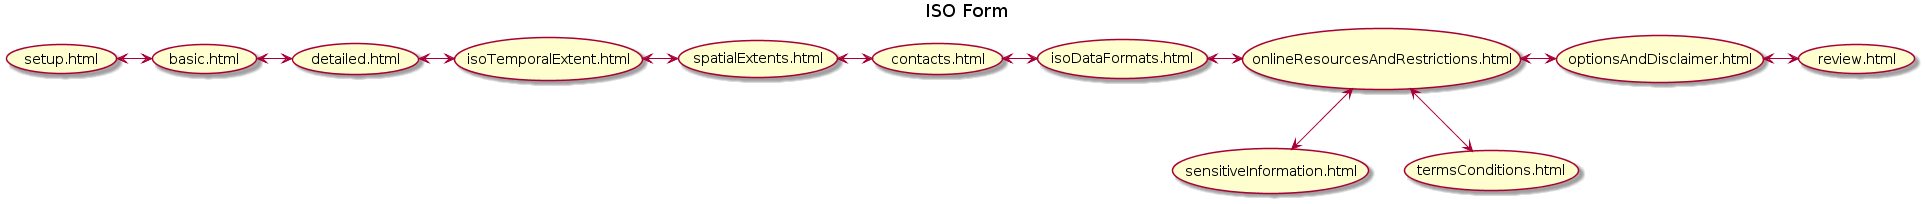
\includegraphics[scale=0.35, angle=-90]{iso-states}

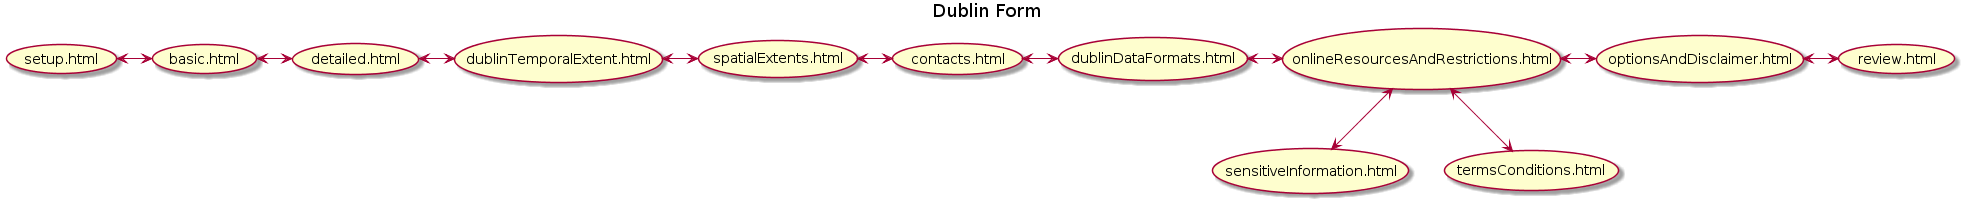
\includegraphics[scale=0.35, angle=-90]{dublin-states.png}

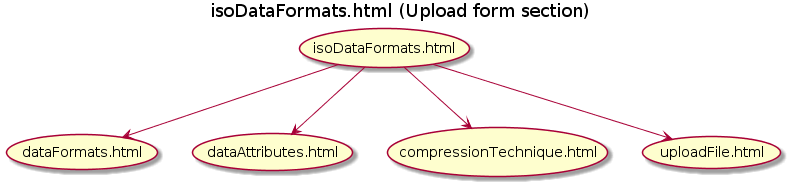
\includegraphics[scale=0.5]{iso-data-formats.png}
\newline

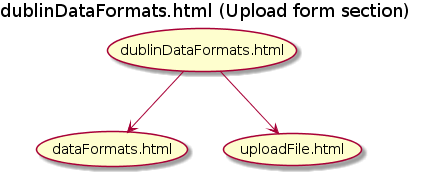
\includegraphics[scale=0.5]{dublin-data-formats.png}
\newline

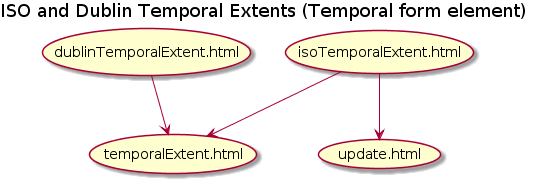
\includegraphics[scale=0.5]{temporal-extent.png}
\newline

\end{document}
